\section{Процентильный интервал}
\footnote{$BC_{a}$ интервал из 14 главы более сложен для объяснения чем процентильный интервал, но не сильно сложне в вычислении. С его помощью можно получить более точные пределы интервала, поэтому он предпочтительнее для практического использования.}Ранее мы обсудили, как можно найти доверительные интервалы используя процентили бутстреп гистограммы. Именно так работает \textit{процентильный интервал}. Предположим, что мы находимся в общей ситуации, показанной на рис. 8.3. Бутстреп выборка $\textbf{x}^{*}$ генерируется в соответствии с $\widehat{P} \rightarrow \textbf{x}^{*}$, и вычисляются бутстреп репликации $\widehat{\theta} = s(\textbf{x}^{*})$. Пусть $\widehat{G}$ --- кумулятивная функция распределения $\widehat{\theta}^{*}$. $1-2\alpha$ процентильный интервал определяется $\alpha$ и $1 - \alpha$ процентилями  $\widehat{G}$:

\begin{gather}\label{13.3}
[\widehat{\theta}_{\%, \text{lo}},\  \widehat{\theta}_{\%, \text{up}}] = [\widehat{G}^{-1}(\alpha),\ \widehat{G}^{-1}(1 - \alpha)].
\end{gather}

Поскольку по определению $\widehat{G}^{-1} = \widehat{\theta}^{*(\alpha)}$, $100\cdot\alpha$ процентный процентиль бутстреп распределения, мы также можем записать процентильный интервал как:
\begin{gather}\label{13.4}
[\widehat{\theta}_{\%, \text{lo}},\  \widehat{\theta}_{\%, \text{up}}] = [\widehat{\theta}^{*(\alpha)},\ \widehat{\theta}^{*(1 - \alpha)}].
\end{gather}
Выражения (\ref{13.3}) и (\ref{13.4}) относятся к идеальной бутстреп ситуации, в которой количество бутстреп репликаций бесконечно. На практике мы должны использовать некоторое конечное число $B$. Генерируем $B$ независимых бутстреп выборок $\textbf{x}^{*1}, \textbf{x}^{*2},...,\textbf{x}^{*B}$ и вычисляем бутстреп репликации $\widehat{\theta} = s(\textbf{x}^{*}), b = 1, 2, ... B$. Пусть $\widehat{\theta}_{B}^{*(\alpha)}$ есть $100\alpha$ эмпирическим процентилем $\widehat{\theta}^{*}(b)$, то есть $B\alpha$ значением в упорядоченном списке
$B$ репликации $\widehat{\theta}$. Итак, если $B = 2000$ и $\alpha = 0.05$, $\widehat{\theta}_{B}^{*(\alpha)}$ это $100$ упорядоченное значение репликаций. (Если $B\cdot \alpha$ не целое число, мы можем использовать соглашение, приведенное после уравнения (\ref{12.22}) в главе 12.) Аналогичным образом $\widehat{\theta}_{B}^{*(1 - \alpha)}$ будет $100\cdot(1-\alpha)$ эмпирическим процентилем. Приблизительный $1 - \alpha$ процентильный интервал:
\begin{gather}\label{13.5}
[\widehat{\theta}_{\%, \text{lo}}, \ \widehat{\theta}_{\%, \text{up}}] \approx [\widehat{\theta}_{B}^{*(\alpha)}, \ \widehat{\theta}_{B}^{*(1 - \alpha)}].
\end{gather}

Если бутстреп распределение $\widehat{\theta}^{*}$ примерно нормальное, то нормальный и процентильный интервалы будут почти совпадать (как на рисунке 13.1). Центральная предельная теорема говорит нам, что при $n \to \infty $ бутстреп гистограмма будет иметь форму нормального распределения, но для небольших выборок она может значительно отличаться от нормально распределённой. Тогда нормальный и процентильный интервалы будут отличаться. Какой из них выбрать для использования?

Обсудим этот вопрос на примере искусственных данных, доверительный интервал которых нам уже известен. Мы сгенерировали выборку $X_{1}, X_{2},...,X_{10}$ из стандартного нормального распределения. Интересующий нас параметр $\theta$ положим равным $e^{\mu}$, где $\mu$ - среднее значение. Истинное значение $\theta$ равно $e^{0} = 1$, в то время как
выборочное значение $\widehat{\theta} = e^{\overline{x}}$ равно 1.25. На левом рисунке 13.2 показана бутстреп гистограмма  $\widehat{\theta}^{*}$ на основе 1000 репликаций (так как мы предполагали что не знаем что выборка имеет нормальное распределение, то использовали непараметрическую бутстреп выборку).

Распределение довольно асимметричное, с длинным хвостом влево. Эмпирические процентили $1000$ $\widehat{\theta}^{*}$ репликаций показаны в таблице 13.2.

\begin{figure}[H]
\center{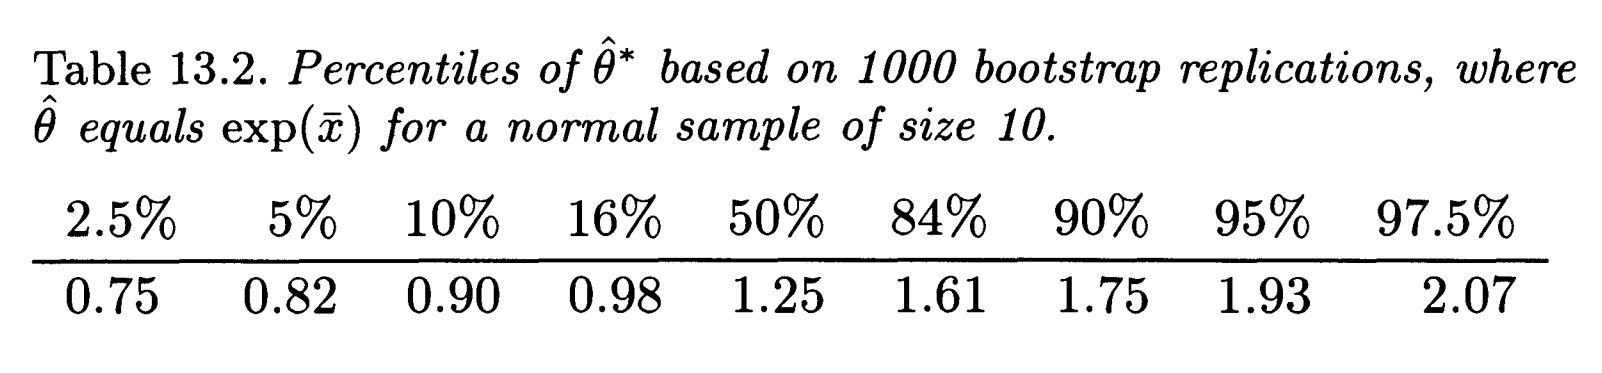
\includegraphics[width=1 \linewidth]{13/t13.4.png}}
\end{figure}

0.95 процентильный интервал  для $\theta$ равен:
\begin{gather}\label{13.6}
[\widehat{\theta}_{\%, \text{lo}}, \ \widehat{\theta}_{\%, \text{up}}] = [0.75, 2.07].
\end{gather}
Будет полезно сравнить его с 0.95 стандартным интервалом на основе $\widehat{\text{se}}_{1000} = 0.34$:
\begin{gather}\label{13.7}
1.25 \pm 1.96\cdot 0.34 = [0.59, 1.92].
\end{gather}

Обратите внимание на большое различие между стандартными нормальными и процентильными интервалами. Есть веская причина предпочесть процентильный интервал (\ref{13.6}) стандартному (\ref{13.7}). Прежде всего отметим, что есть очевидное возражение против (\ref{13.7}). Левый рисунок 13.2 показывает, что нормальное приближение $\widehat{\theta} \sim \mathrm{N}(\theta, \widehat{\text{se}}^{2})$, лежащее в основе стандартных интервалов, в данном случае не очень точное. Логарифмическое преобразование преобразует распределение $\theta$ в нормальное. На правом рисунке 13.2 изображена бутстреп гистограмма для 1000 значений $\widehat{\varphi}^{*} = \log(\widehat{\theta}^{*})$, а также стандартный нормальный и процентильный интервалы для $\varphi$. Обратите внимание, что гистограмма гораздо ближе к нормальному распределению, чем гистограмма для $\widehat{\theta}^{*}$. Это неудивительно, поскольку  $\widehat{\varphi}^{*} = \overline{x}^{*}$. Стандартный нормальный интервал для $\varphi = \log(\theta)$ равен $[-0.28,\ 0.73]$, а процентильный интервал $[-0.29,\ 0.73]$. Из-за нормальной формы гистограммы эти интервалы согласуются лучше, чем на левом рисунке. Поскольку гистограмма на правом рисунке 13.2 ближе, чем на левом, к нормальному закону, разумнее сторить интервал основываясь на $\widehat{\varphi}$, а не на $\widehat{\theta}$, а затем отбразить граничные точки обратно в тот же масштаб что и $\theta$.

\begin{figure}[H]
\center{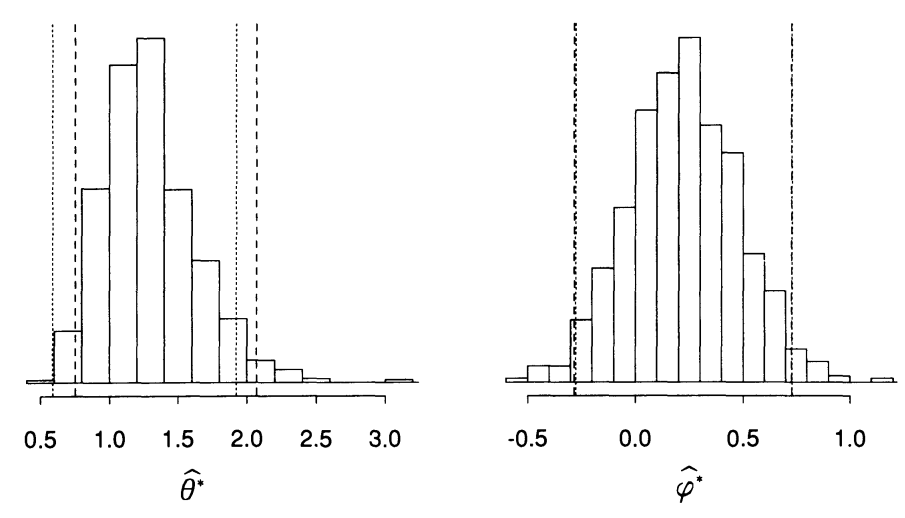
\includegraphics[width=1 \linewidth]{13/f13.5.png}}
\end{figure}

Обратная к логарифму функция это экспоненента. После применения экспоненциальной функции для отображения стандартного интервала обратно в шкалу $\theta$ получим интервал $[0.76, 2.08]$. Этот интервал ближе к процентильному интервалу $[0.75, 2.07]$, нежели стандартный интервал $[0.59, 1.92]$, построенный с использованием $\widehat{\theta}$ напрямую.

Мы видим, что процентильный интервал для $\theta$ хорошо согласуется со стандартным нормальным интервалом, который был построен с помощью преобразования $\theta$, а затем обратно преобразованный в шкалу $\theta$. Сложность в улучшении стандартного метода заключается в том, что нам нужно знать другое преобразование, например логарифм, для каждого интересующего нас параметра $\theta$. Метод процентилей можно рассматривать как алгоритм для автоматического объединения таких преобразований.

Следующий результат формализует тот факт, что метод процентилей всегда <<знает>> правильное преобразование:

\underline{Лемма о процентильном интервале}. Предположим, что преобразование $\widehat{\varphi} = m(\widehat{\theta})$ полностью нормализует распределение $\theta$:
\begin{gather}\label{13.8}
\widehat{\varphi} \sim \mathrm{N}(\varphi, c^{2}),
\end{gather}
для некоторого отклонения c. Тогда процентильный интервал на основе $\widehat{\theta}$ равен $[m^{-1} (\widehat{\varphi}- z^{(1 - \alpha)}c), m^{-1} (\widehat{\varphi}- z^{(\alpha)}c)]$.

В схеме на рис. 8.3 в 8 главе, где вероятностный механизм $P$, связанный с параметром $\theta$, дает данные $\textbf{x}$. Мы предполагаем, что  $\widehat{ \varphi} = m(\widehat{\theta})$ и  $\varphi = m(\theta)$ удовлетворяют (\ref{13.8}) для любого $P$. В этом предположении лемма не более чем утверждение, о том что метод процентилей правильно преобразует конечные точки. См. Задачи 13.1 и 13.2.

Читатель может думать о методе процентилей как о вычислительном алгоритме для расширения диапазона эффективности стандартных интервалов. В ситуациях, подобных той что на рис. 13.1, $\widehat{\theta} \sim \mathrm{N}(\theta,\ \widehat{\text{se}}^{2})$, где стандартные интервалы почти точны, процентильные интервалы согласуются с ними. В ситуациях, подобных ситуации на левом рисунке 13.2, где стандартные интервалы были бы правильными, если бы мы преобразовали параметры $\theta$ в $\varphi$, метод процентилей автоматически выполняет это преобразование. Преимущество метода процентилей в том, что нам не нужно знать правильное преобразование. Все, что мы предполагаем, это то, что такое преобразование существует.

В начале 1920-х годов Рональд Фишер разработал теорию максимального правдоподобия, которая автоматически даёт эффективные оценки для $\widehat{\theta}$ и стандартной ошибке $\widehat{\text{se}}$ в самых разных ситуациях. (В главе 21 обсуждается тесная связь между теорией максимального правдоподобия и бутстрепом.) Теория Фишера значительно расширила использование стандартных интервалов, облегчив их вычисление, и улучшев их обоснование. С тех пор статистики разработали множество уловок для улучшения практических характеристик стандартных интервалов. Среди них список преобразований, которые делают определенные типы задач более подходящими для идеальной ситуации  $\widehat{\theta} \sim \mathrm{N}(\theta, \ \widehat{\text{se}}^{2})$. Процентильный интервал расширяет пользу от использования стандартного нормального интервала, не требуя явного знания этого списка преобразований.